\documentclass[
    ../../Software_Engineering_Summary.tex,
]
{subfiles}

\externaldocument[ext:]{../../Software_Engineering_Summary.tex}
% Set Graphics Path, so pictures load correctly
\graphicspath{{../../}}

\begin{document}
\section{Software Development Process}
\subsection{Introduction}
The \defc{software development process} is a set of activities and associated results that produce a software product.

\begin{defbox}
    [Fundamental Process Activities]
    \begin{tabularx}{\textwidth}{r X}
        \defc{Software specification:} & \textbf{Definition} of the software to be produced and the constraints of the operation\\
        \defc{Software development:} & \textbf{Design}, \textbf{implementation}, \textbf{verification} of the software\\
        \defc{Software validation:} & \textbf{Ensure} that the software behaves according to the \textbf{requirements}\\
        \defc{Software evolution:} & \textbf{Adaptation} and \textbf{modification} of the software to cope with changing requirements\\
    \end{tabularx}
\end{defbox}

\subsubsection{Motivation}
\begin{defbox}
    [Size of the Task]
    Organize a potentially large team
    \begin{itemize}
        \item Assign responsibilities
        \item Define modes of collaboration
    \end{itemize}
\end{defbox}

\begin{defbox}
    [Complexity of the Task]
    Many different kinds of activities
    \begin{itemize}
        \item Dependencies among tasks, when to do what
    \end{itemize}
\end{defbox}

\begin{defbox}
    [Quality Control]
    Need to be able to know whether things go wrong or right
\end{defbox}

\subsubsection{Software Engineering Process Models}
\defc{Software Engineering Process Models} are simplified and abstract descriptions of software processes that present \defc{one view} of that process. 

They may include activities that are part of the software process, software products (e.g. architectural descriptions, source code, documentation\dots) and the \defc{roles} of people involved in software engineering.

Large projects may use different, multiple software process models to develop different parts of the software.

\newpage
\subsection{Waterfall Model}
The \defc{waterfall model} is a \defc{linear} development process model that has the following phases:

\begin{defbox}
    [Waterfall Phases]
	\begin{enumerate}
        \item \defc{Requirements Analysis and Definition:}
        \begin{itemize}
            \item Requirements are established by consultation with system users
            \item \textbf{Requirements are defined in detail and serve as system specification}
        \end{itemize}
        \item \defc{System and Software Design:}
        \begin{itemize}
            \item Definition of the overall system \defc{architecture}
            \item Identification of the \defc{fundamental abstractions} and their relations
        \end{itemize}
        \item \defc{Implementation and Unit Testing:}
        \begin{itemize}
            \item Software design is realizes as a set of \defc{program units}
            \item \defc{Testing} verifies that each unit meets its specification.
        \end{itemize}
        \item \defc{Integration and System Testing:}
        \begin{itemize}
            \item Program units are \defc{integrated} and tested as a complete system
        \end{itemize}
        \item \defc{Operation and Maintenance}
    \end{enumerate}
\end{defbox}

\begin{minipage}
    [c]{0.45\textwidth}
    \begin{itemize}
        \item The result of each phase is a set of approved artifacts
        \item Following phase start \defc{after} the previous one is finished
        \item In case of errors the previous phases are \defc{repeated}
        \item Aligns with traditional (physical) engineering process models
    \end{itemize}
\end{minipage}
\begin{minipage}
    [c]{0.55\textwidth}
    \centering
    \includegraphics[width = 0.8\textwidth]{Pics/13/WaterfallModel.png}
\end{minipage}

\subsubsection{Criticism}
The waterfall model in general does not work well for software engineering.
\begin{itemize}
    \item \defc{Not iterative:} early prototyping is not possible
    \item \defc{Change} of requirements, design\dots difficult 
    \begin{itemize}
        \item Major Changes are undesirable, even minor changes are expensive
    \end{itemize}
    \item \defc{Testing} starts only at the later stages
    \item \defc{Different phases} executed by \defc{different teams}
    \begin{itemize}
        \item Might no longer be available once a phase is finished
    \end{itemize}
\end{itemize}

\newpage
\subsubsection{V-Model}
The V-Model is closely related to the waterfall method.

\begin{minipage}
    [c]{0.4\textwidth}
    As a result most of the criticism of the waterfall method carries over.
    \begin{itemize}
        \item Not iterative
        \item Change of requirements expensive
    \end{itemize}

    Should only be used when:
    \begin{itemize}
        \item Project requirements \defc{stable} and \defc{well-known}
        \item \defc{Small, short} project
        \item \defc{Very precise and detailed} requirements and documentation (e.g. safety critical, like medical devices, avionics\dots)
    \end{itemize}
\end{minipage}
\begin{minipage}
    [c]{0.6\textwidth}
    \centering
    \includegraphics[width = \textwidth]{Pics/13/VModel.png}
\end{minipage}

\subsection{Agile Development}
Agile development is \defc{centered on maintenance}.

\begin{defbox}
    [Goal]
    Develop software \defc{quickly} in presence of \defc{rapidly changing} requirements 
\end{defbox}

Development cycles should be small and fast: \defc{agile}.

Originally for small teams (3-9 teams members).

\subsubsection{Requirements}
\begin{itemize}
    \item Analyst, \defc{customer}, developer, tester etc. work together as a team
    \begin{itemize}
        \item Necessitates that all role players are always available
    \end{itemize}
    \item Employ practices that provide necessary \defc{discipline} and \defc{feedback}
    \item Employ desing principles that keep software \defc{flexible} and \defc{maintainable}
\end{itemize}

Agility is not a substute for validation: Customer \defc{must} commit to become a team member

\subsubsection{Manifesto}
\begin{defbox}
    [1: Individuals and Interactions over Process and Tools]
    The best tools will not help, if your team does not work together.

    \begin{minipage}
        [c]{0.4\textwidth}
        Team size should start small - Grow or shrink as needed
    \end{minipage}
    \begin{minipage}
        [c]{0.6\textwidth}
        \centering
        \includegraphics[width = 0.6\textwidth]{Pics/13/Manifesto1Groupsize.png}
    \end{minipage}

    \begin{minipage}
        [c]{0.4\textwidth}
        Workload should be sustainable: No bursts
    \end{minipage}
    \begin{minipage}
        [c]{0.6\textwidth}
        \centering
        \includegraphics[width = 0.6\textwidth]{Pics/13/Manifesto1Workload.png}
    \end{minipage}

    Team should regularly reflect on process, work environment\dots
\end{defbox}

\begin{defbox}
    [2: Working Software over Comprehensive Documentation]
    System structure and rationales for the design should be documented, but \defc{incremental} rather than upfront.

    Not an excuse for \defc{lack of documentation}, simply a recommendation of workflow. In agile development, code plays a central role so it must be \defc{even better} documented than elsewise.
\end{defbox}

\begin{defbox}
    [3: Customer Collaboration over Contract Negotiation]
    Contract should specify how the collaboration between development team and customer looks like.

    A contract that merely specifies payment and delievery is \defc{not enough}, a customer wants an idea of what their money is doing.
\end{defbox}

\begin{defbox}
    [4: Responding to Change over Following a Plan]
    A plan outlined at the beginning of the project might be followed less and less over time, as requirements change and make the plan suboptimal. Sticking to a rigid plan might be counterproductive.

    \begin{center}
        \includegraphics[width = 0.7\textwidth]{Pics/13/Manifesto4Plan.png}
    \end{center}
\end{defbox}

\subsubsection{Agile Processes}
\begin{figure}
    [H]
    \centering
    \includegraphics[width = \textwidth]{Pics/13/AgileProcesses.png}
    \includegraphics[width = 0.6\textwidth]{Pics/13/AgileProcessesLegend.png}
\end{figure}

\newpage
\subsection{Extreme Programming (XP)}
XP is composed of a set of simple, interdependent elements / practices.

\subsubsection{Practices \& Elements}
\begin{defbox}
    [Element: Customer]
    \begin{itemize}
        \item Defines and prioritizes features
        \item A member of the team and available to the team
    \end{itemize}
\end{defbox}

\begin{defbox}
    [Practice: User Story]
    \begin{itemize}
        \item Requirements identified in discussion with the customer
        \item Very concise (succinct) text with an estimate of its relative difficulty
        \item Almost no details, technical details likely to change anyway
    \end{itemize}

    \hrule
    \vspace{5pt}
    \begin{center}
        \defc{Good User Story:}
    \end{center}
    \begin{defbox}
        [Template]
        \begin{tabularx}
            {\textwidth}{p{0.2\textwidth} X}
            \defc{Long Template:} & As a <Role>, I want <Goal> so that <Reason> \\
            \defc{Short Template:} & As a <Role>, I want <Goal> \\
        \end{tabularx}
    \end{defbox}

    \begin{defbox}
        [Characteristics]
        Each story must
        \begin{itemize}
            \item be understandable to the customer
            \item provide something of value to the customer
            \item be sized so that several can be implemented per iteration
            \item be independent
            \item be testable
        \end{itemize}
    \end{defbox}

    Work according to the \defc{INVEST} principle:
    \begin{itemize}
        \item \defc{I}ndependent:
        \begin{itemize}
            \item Self-contained, \defc{no inherent dependency} on other stories
        \end{itemize}
        \item \defc{N}egotiable:
        \begin{itemize}
            \item User Stories can always be \defc{changed} and \defc{rewritten} (up until a \defc{sprint})
        \end{itemize}
        \item \defc{V}alueable:
        \begin{itemize}
            \item Must deliver \defc{value} to the end user
        \end{itemize}
        \item \defc{E}stimable:
        \begin{itemize}
            \item Possible to \defc{estimate} size (implementation effort) of story
        \end{itemize}
        \item \defc{S}ized appropriately (or \defc{S}mall):
        \begin{itemize}
            \item Not as big as impossible to plan/prioritize with certainty
        \end{itemize}
        \item \defc{T}estable:
        \begin{itemize}
            \item Contain enough information to enable \defc{test design}
        \end{itemize}
    \end{itemize}
\end{defbox}

\begin{defbox}
    [Element: Acceptance Test]
    Details of user stories are captured in the form of \defc{acceptance tests}.

    Acceptance tests are written before or concurrently with the implementation of a user story.

    Once a test passes, it is added to the set of passing acceptance tests and is never allowed to fail again. (Avoid \defc{regression})
\end{defbox}

\begin{defbox}
    [Practice: Short Development Cycles]
    \defc{Sprint / Iteration:} A fixed sized time interval in which a set of software features is implemented. 

    At the end of each sprint is a piece of executable software that can be tested - may or may not be deployed into production.

    \defc{Time Boxed:} Not extended if planned features cannot be implemented in time - In this case, features must be \defc{moved} to a later iteration

    \begin{center}
        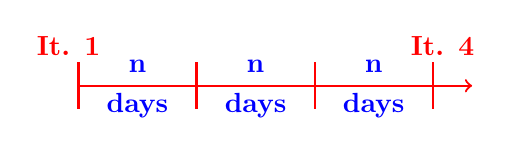
\begin{tikzpicture}
            % Draw the timeline
            \draw[->, thick, red] (0,0) -- (5,0);
        
            % Draw interval divisions
            \foreach \x in {0,1.5,3,4.5} {
                \draw[thick, red] (\x,0.3) -- (\x,-0.3);
            }
        
            % Labels for iterations
            \node[red] at (-0.125,0.5) {\textbf{It. 1}};
            \node[red] at (4.625,0.5) {\textbf{It. 4}};
        
            % Interval labels
            \foreach \x in {0.75,2.25,3.75} {
                \node[blue] at (\x,0.25) {\textbf{n}};
            }
        
            % "days" labels
            \foreach \x in {0.75,2.25,3.75} {
                \node[blue] at (\x,-0.25) {\textbf{days}};
            }
        
        \end{tikzpicture}
    \end{center}
\end{defbox}

\begin{defbox}
    [Practice: Planning Game]
    Division of responsibility between business and development

    \defc{Business people} decide the \defc{importance} of a feature,\\
    \defc{developers} decide how much that feature will \defc{cost} to implement.

    \begin{center}
        \begin{tikzpicture}
            % Draw the timeline
            \draw[->, thick, red] (0,0) -- (5,0);
        
            % Draw interval divisions
            \foreach \x in {0,1.5,3,4.5} {
                \draw[thick, red] (\x,0.3) -- (\x,-0.3);
            }
        
            % Labels for iterations
            \node[red] at (-0.125,0.5) {\textbf{It. 1}};
            \node[red] at (4.625,0.5) {\textbf{It. 4}};
        
            % Interval labels
            \foreach \x in {0.75,2.25,3.75} {
                \node[blue] at (\x,0.25) {\textbf{n}};
            }
        
            % "days" labels
            \foreach \x in {0.75,2.25,3.75} {
                \node[blue] at (\x,-0.25) {\textbf{days}};
            }

            \foreach \x in {0.75,3.75} {
                \node[codegreen] at (\x,1) {\textbf{Feature}};
            }

            \foreach \x in {0.75,3.75} {
                \node[codegreen] at (\x,0.7) {\textbf{X,Y\dots}};
            }

            \foreach \x in {2.25} {
                \node[codegreen] at (\x,0.8) {\textbf{\dots}};
            }
        
        \end{tikzpicture}
    \end{center}
\end{defbox}

\begin{defbox}
    [Practice: Simplicity]
    Make the design as \defc{simple} and \defc{expressive} as possible. 

    Focus on \defc{current} set of user stories - do not worry about \defc{future} ones.
\end{defbox}

\begin{defbox}
    [Element: Test-Driven Development (TDD)]
    \begin{center}
        \defc{Implementation starts with writing tests}
    \end{center}
    \defc{Afterwards} the actual feature / functionality is implemented

    Any code is written to make failing tests (unit) \defc{tests pass}.

    Tests are written by:
    \begin{itemize}
        \item \defc{Developers:} (unit tests)
        \item \defc{Customers:} (functional / acceptance tests) 
    \end{itemize}
\end{defbox}

\begin{defbox}
    [Practice: Continous Integration]
    Programmers commit their code and integrate their work \defc{several times per day} - non blocking version of version control

    \defc{After each commit:} System is built and every test (incl. acceptance) is run

    \hrule
    \vspace{5pt}
    \defc{Requirements:}
    \begin{itemize}
        \item Usage of version control system (git, svn, etc.)
        \item Automated build system
        \item Automated test execution
    \end{itemize}
\end{defbox}

\begin{defbox}
    [Element: Refactoring]
    Improve program structure \defc{without changing} existing behaviour.

    Refactor \defc{frequently} to avoid code ''rots'' due to adding feature after feature.

    Before adding a feature refactoring should be considered.
\end{defbox}

\begin{defbox}
    [Practice: Pair Programming]
    Programmers \defc{pair up} to write code:
    \begin{itemize}
        \item One focuses on the \defc{best way} to implement a feature
        \item The other looks at the ocde being written, but from \defc{strategic} point of view
    \end{itemize}

    Pairing changes often to \defc{spread knowledge.}

    \vspace{5pt}
    \defc{Requirements:}
    \begin{itemize}
        \item Programmers must be at a \defc{comparable skill level}
        \item Must \defc{subdue proprietary impulses} to ''own'' code
    \end{itemize}
\end{defbox}

\begin{defbox}
    [Practice: Collective Ownership]
    \defc{Team owns the code} - any pair has the right to check out any module.

    Everyone takes over responsibility for the whole system - no single person is blamed for problems
\end{defbox}

\begin{defbox}
    [Element: Coding Standards]
    Establish appropriate coding standards:
    \begin{itemize}
        \item Promote \defc{least} amount of work possible
        \item Respect ''\defc{no duplicate code}'' principle
        \item Emphasize \defc{communication}
        \item \defc{Accepted} by whole team
    \end{itemize}
\end{defbox}

\subsubsection{Planning}
\begin{defbox}
    [Initial Exploration (Start of the project)]
    \begin{itemize}
        \item Developer \& customers identify all \defc{significant} user stories (not all user stories)
        \item Developers estime the stories relative to each other using \defc{story points} (how long it'll take to implement)
        \item Actual size determined by \defc{velocity} (= story points of previous iteration, initially just a guess, gains accuracy as iterations progress)
    \end{itemize}
\end{defbox}

\begin{defbox}
    [Release Planning]
    \begin{itemize}
        \item Developers \& Customer agree on date for \defc{first release} (2-4 months)
        \item Customer \defc{picks} stories and rough \defc{order} (limited by velocity)
        \item As velocity gains accuracy, \defc{adjust release plan} (number of stories)
    \end{itemize}
\end{defbox}

\begin{defbox}
    [Iteration Planning]
    \begin{itemize}
        \item Customer picks stories for iteration n (must not exceed velocity of iteration n - 1)
        \item Within one iteration the \defc{order} is a technical decision
        \item Iteration ends on specified date (\defc{time-boxed}, even when not all stories finished)
        \item Compute \defc{velocity} of completed iteration: Sum of estimates of all \defc{successfully finished} stories
        \item \defc{Planned velocity} for iteration n + 1:= \defc{Measured velocity} of iteration n
    \end{itemize}
\end{defbox}

\begin{defbox}
    [Task Planning]
    Stories broken down into tasks of 4 - 16 hours implementation time

    Developers choose tasks freely
\end{defbox}

\subsubsection{Additional Remarks on Processes}
\begin{defbox}
    [Different Types of Systems Need Appropriate Processes]
    \begin{itemize}
        \item Software running an aircraft developed using different process than an e-commerce website
        \item Operating system developed differently than a word processor
        \item In large systems different parts may be developed using different processes
    \end{itemize}
\end{defbox}

\begin{defbox}
    [No Be-All-End-All Process Model]
    Processes must use the capabilities of the \defc{people} in an organization

    Processes must follow the specific \defc{characteristics} of the developed software
\end{defbox}
\end{document}